\subsection{Gravity and General Relativity} 

(Answers to M\Alph{subsection} problems are on page \pageref{gravity_prob_answers}.)


\begin{Exercise}[difficulty=0]
Suppose that you are closed inside a rocket with no windows, and no instruments except for a simple bathroom scale to stand on.  Now consider two scenarios drawn below: In scenario A, the rocket is at rest on the surface of the Earth, where the gravitational constant is $g=9.8~{\rm m/s}^2$. In scenario B, the rocket is far away from any stars or planets in interstellar space, and its engines are accelerating the rocket forwards at $a=g=9.8~{\rm m/s}^2$.
\begin{center}
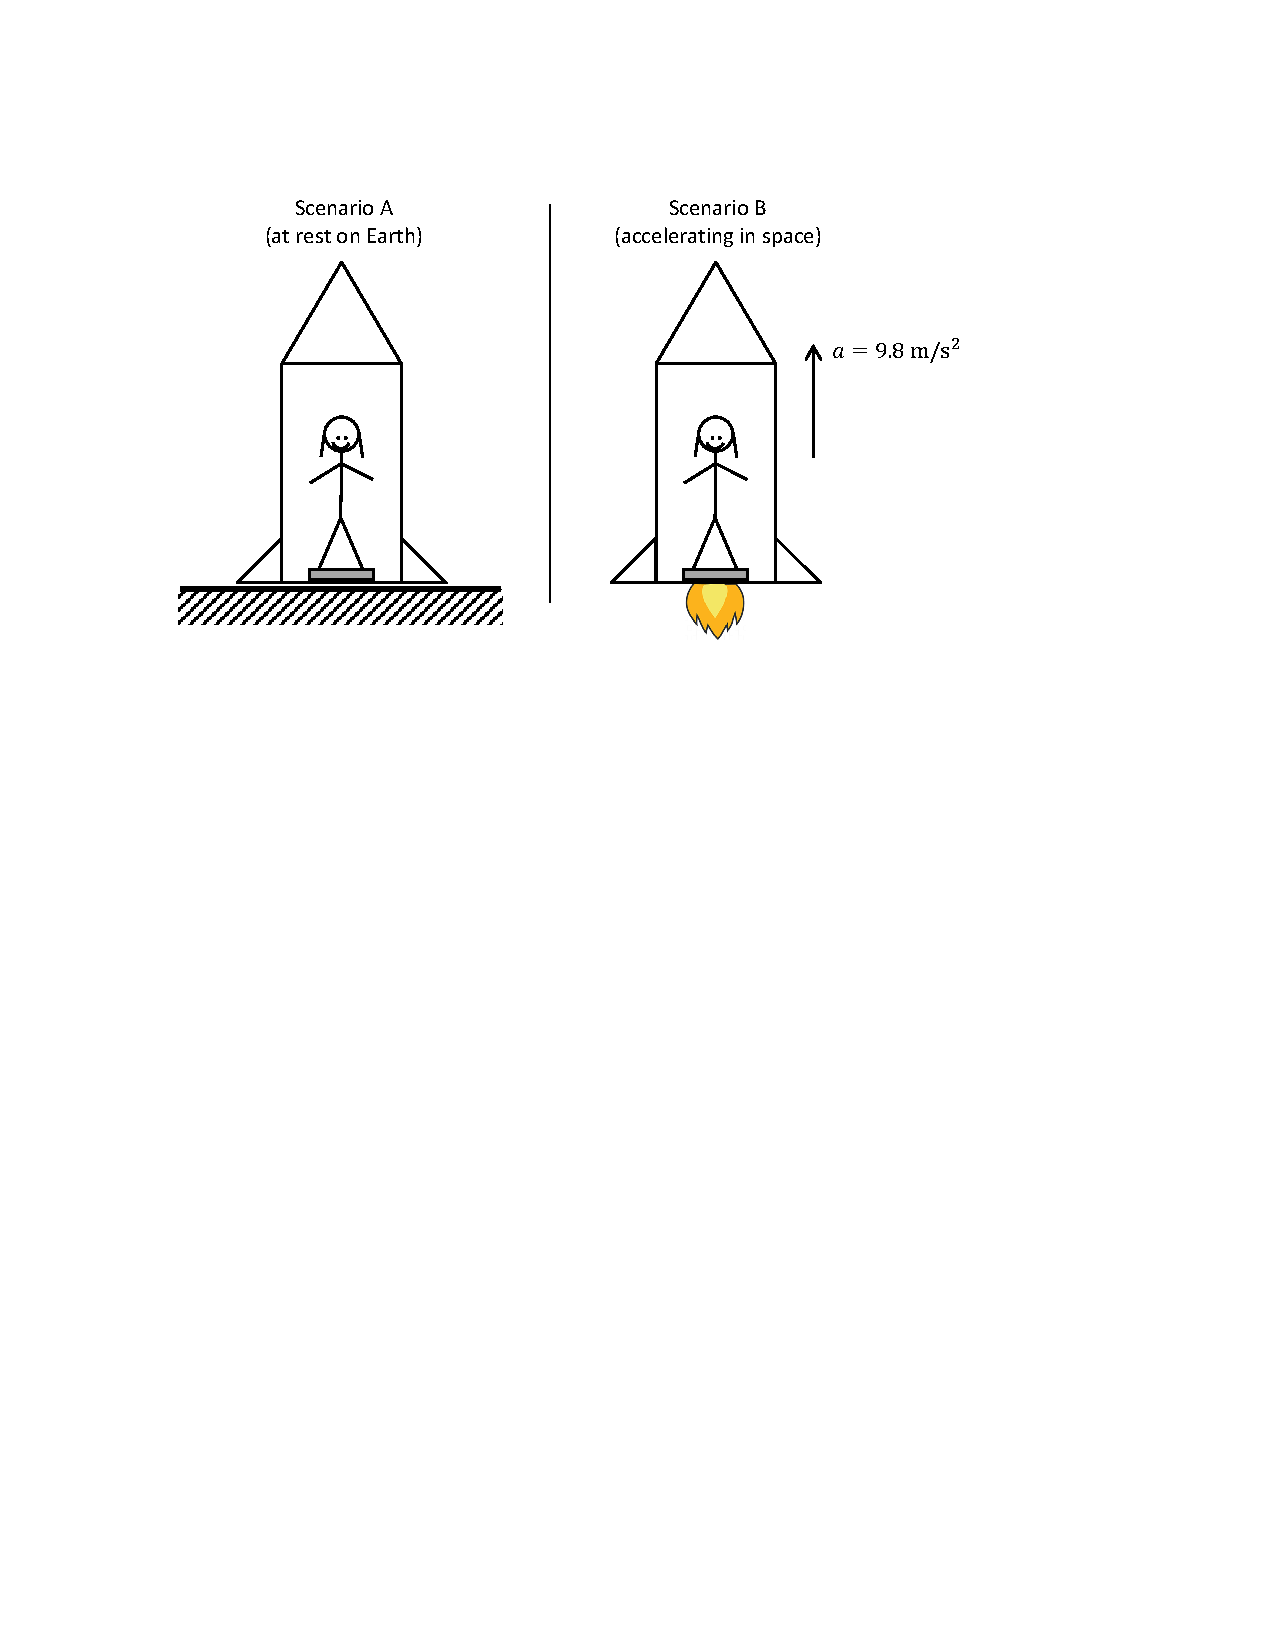
\includegraphics[scale=0.9]{M_problems/gravity/two_rockets_equivalence.pdf}
\index{color page}
\end{center}
(a) Draw a free-body diagram of \textit{you} in scenario A, and a free-body diagram of \textit{you} in scenario B.  In each case, draw vectors showing only the forces that are acting \textit{on you, directly,} not on the rocket ship.  (b)~If you were not told what situation you were in, could you tell the difference by standing on the bathroom scale and reading your ``weight''?  (c)~Suppose the engines were very, very quiet, so you could not hear or see whether they were on.  Would scenario A feel any different from scenario B?  If yes, how would it feel different?
\end{Exercise}


\begin{Exercise}[difficulty=0]
Congratulations!  You entered a raffle and have just won first prize: a one-week trip to Denver!\,\footnote{Second prize: two weeks.}  The elevation in Denver is roughly 1600 meters above sea level, hence its nickname, ``the mile-high city.''  If you spend a week in Denver, who ages more: you, or your friend who stays in Richmond? (Richmond is essentially at sea level.)  How large is this difference?
\end{Exercise}
\begin{Answer}
You age more than your friend in Richmond, and the difference you calculate should be close to 100 nanoseconds.
\end{Answer}

\begin{Exercise}[difficulty=0]
A very accurate atomic clock is placed on a jet plane, and an identical clock remains stationary on the ground.  The clock on the plane flies away from the stationary clock for five hours at the plane's standard cruise speed of 250~m/s at an altitude of 13000 m, then makes a U-turn and returns at the same speed and altitude.  What would be the difference in time measured between the two clocks at the end of the trip (a)~considering only time dilation related to the speed of the aircraft (special relativity), (b)~considering only time dilation due to gravity (general relativity), and (c)~considering both special and general relativity?  (d)~Which is the greater effect?
\end{Exercise}
\begin{Answer}
(a) 12.5 ns (b) 51 ns (c) 38.5 ns
\end{Answer}


\begin{Exercise}[difficulty=0]
\label{how_far_does_rocket_travel_prob}
In the example we did in class, we imagined a rocket with a light source at the bottom, and you as an observer at the top.  Suppose the rocket had a height of $H=20$~meters.  (a)~How long would it take light to travel the length of the rocket?  (b)~At an acceleration of $a=9.8~{\rm m/s}^2$, what would be the final speed of the rocket once the light reaches the top of the rocket, assuming the rocket starts at rest ($v=0$)?  (c)~What is the rocket's average speed during this time?  (Just $(v_{\rm initial} +v_{\rm final})/2$, that's all.)  (d)~At that average speed, how far does the rocket travel during this time?  (e)~In Activity 2 of Lab~\ref{gravity_time_lab}, we assumed that we could still treat the distance traveled by the light in our example as being approximately equal to the height of the rocket $H$.  Is that a reasonable approximation? 
\end{Exercise}
\begin{Answer}
(a) 66 ns (b) $6.5 \times 10^{-7}$~m/s (c) $3.27 \times 10^{-7}$ m/s (d) About 22 femtometers
\end{Answer}


\begin{minipage}{0.75 \textwidth}
\begin{Exercise}[difficulty=0]
A laser beam inside of a rocket ship is aimed exactly horizontally from one side of the ship to the other, hitting the opposite wall 4~meters away.  (a)~Suppose the ship is floating in space ($v=0$ in some reference frame), far away from any gravitational source.  At the moment the laser beam is turned on, the ship's engines fire, accelerating the ship forward at $a=9.8~{\rm m/s}^2$.  By what distance has the ship moved forward in the time it takes for the laser beam to cross the 4-meter width of the ship? (Hint: your work in Problem \ref{how_far_does_rocket_travel_prob} will be helpful here.)  (b)~Now suppose instead that the ship is standing motionless on the surface of the Earth.  By what vertical distance is the laser beam deflected down by the Earth's gravitational field?
\vspace{0.5in}
\end{Exercise}
\end{minipage}
\begin{minipage}{0.24 \textwidth}
\medskip
\hspace{\fill}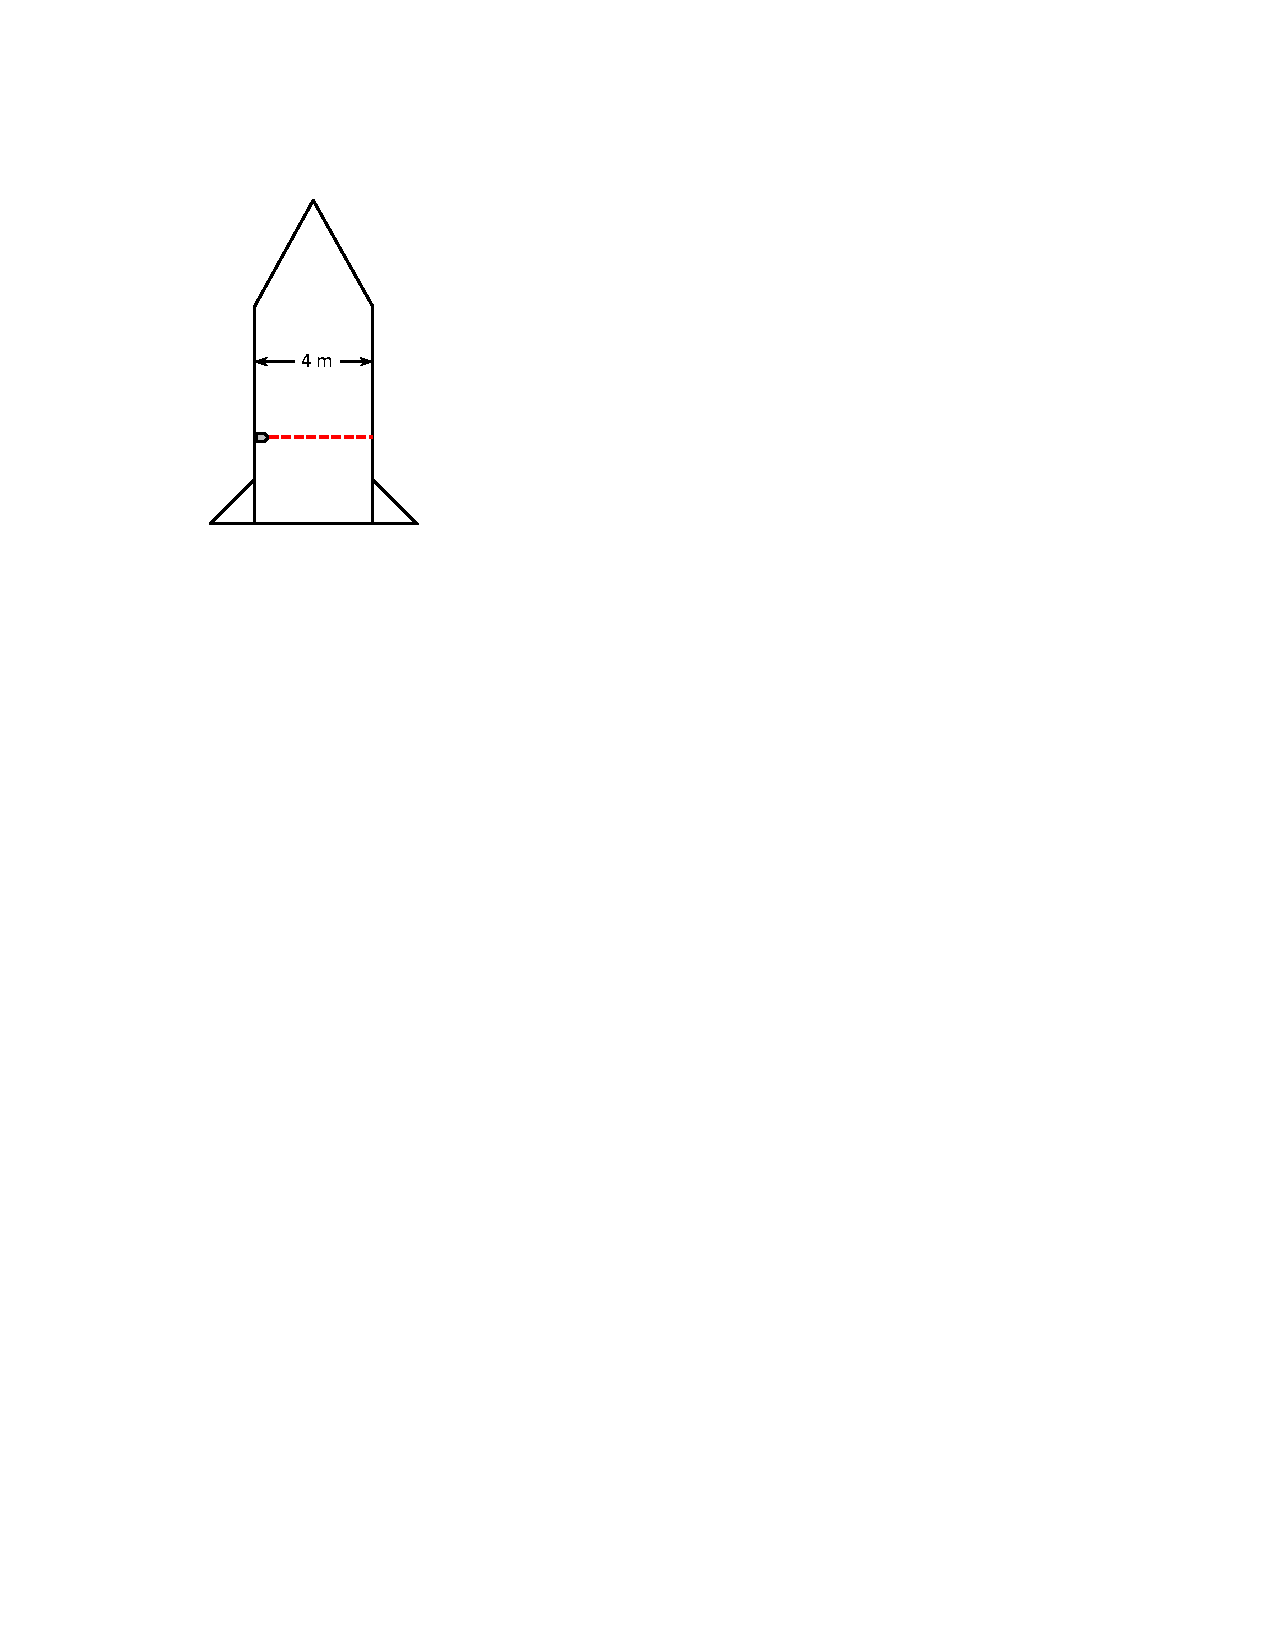
\includegraphics[scale=0.9]{M_problems/gravity/rocket_and_horizontal_laser.pdf}
\index{color page}
\end{minipage}
\begin{Answer}
(b) 0.88 femtometers
\end{Answer}





\bigskip\bigskip\bigskip
\pagebreak[3]
\textbf{Answers to Selected {\thesubsection} Problems:}
\label{gravity_prob_answers}
%\shipoutExercise
\shipoutAnswer

\cleardoublepage